\documentclass[border=1pt]{standalone}
\usepackage[dvipsnames]{xcolor}
\usepackage{tikz}                       % Graphen und kommutative Diagramme
\usetikzlibrary{patterns}               % Um schraffierte Formen in der tikzpicture-Umgebung zu zeichnen.

\begin{document}

\newcommand{\ul}{\underline}


\centering
\begin{minipage}{.55\textwidth}
\centering
\resizebox{!}{4.3cm}{
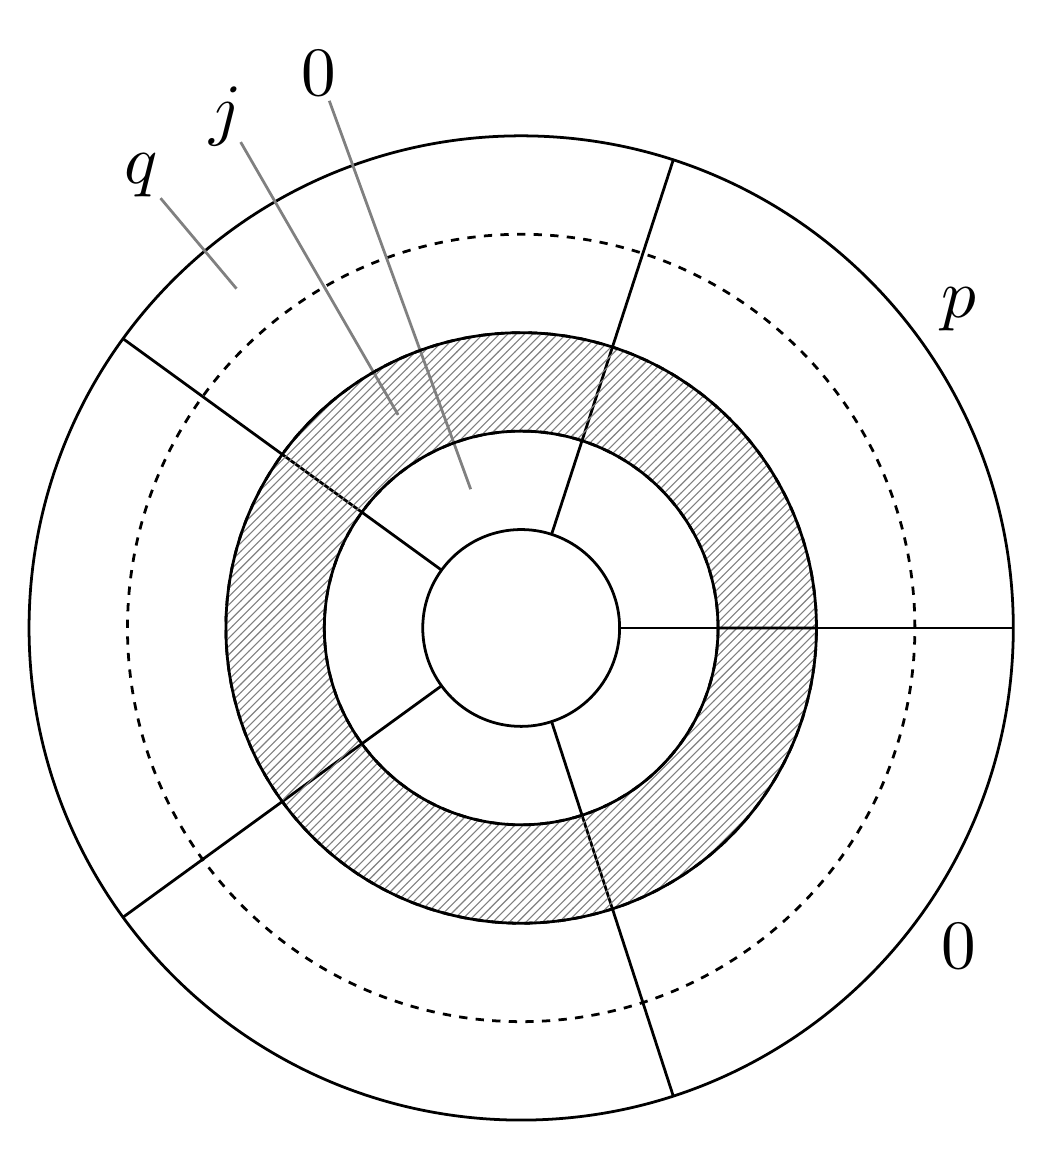
\begin{tikzpicture}[x=1.25cm, y=1.25cm, line width=1pt]

% draw inner and outer circle
\draw[color=black] (0, 0) circle (1);
\draw[color=black] (0, 0) circle (5);

% draw dashed circles
\foreach \i in {2,...,4}
{
    \draw[color=black, dashed] (0, 0) circle (\i);
}

% draw radial lines
\foreach \i in {0,...,4}
{
		\draw (\i * 72 : 1) -- (\i * 72 : 5);
}

%draw nodes
\draw node[scale = 2.5] at (110 : 6) {$0$};
\draw[color=black!50] (110 : 5.7) -- (110 : 1.5);
\draw node[scale = 2.5] at (120 : 6) {$j$};
\draw[color=black!50] (120 : 5.7) -- (120 : 2.5);
\draw node[scale = 2.5] at (130 : 6) {$q$};
\draw[color=black!50] (130 : 5.7) -- (130 : 4.5);

\draw node[scale = 2.5] at (72 * 4 + 36 : 5.5) {$\ul 0$};
\draw node[scale = 2.5] at (36 : 5.5) {$\ul p$};

% draw shaded concentrical stripe
\filldraw[pattern=north east lines, pattern color=gray] (2, 0) arc [radius = 2, start angle = 0, delta angle = 360]
                                                     -- (3, 0) arc [radius = 3, start angle = 0, delta angle = -360]
                                                     -- cycle;
\end{tikzpicture}
}
\end{minipage}
\hspace{1cm}
\begin{minipage}{.55\textwidth}
\centering
\resizebox{!}{4.3cm}{
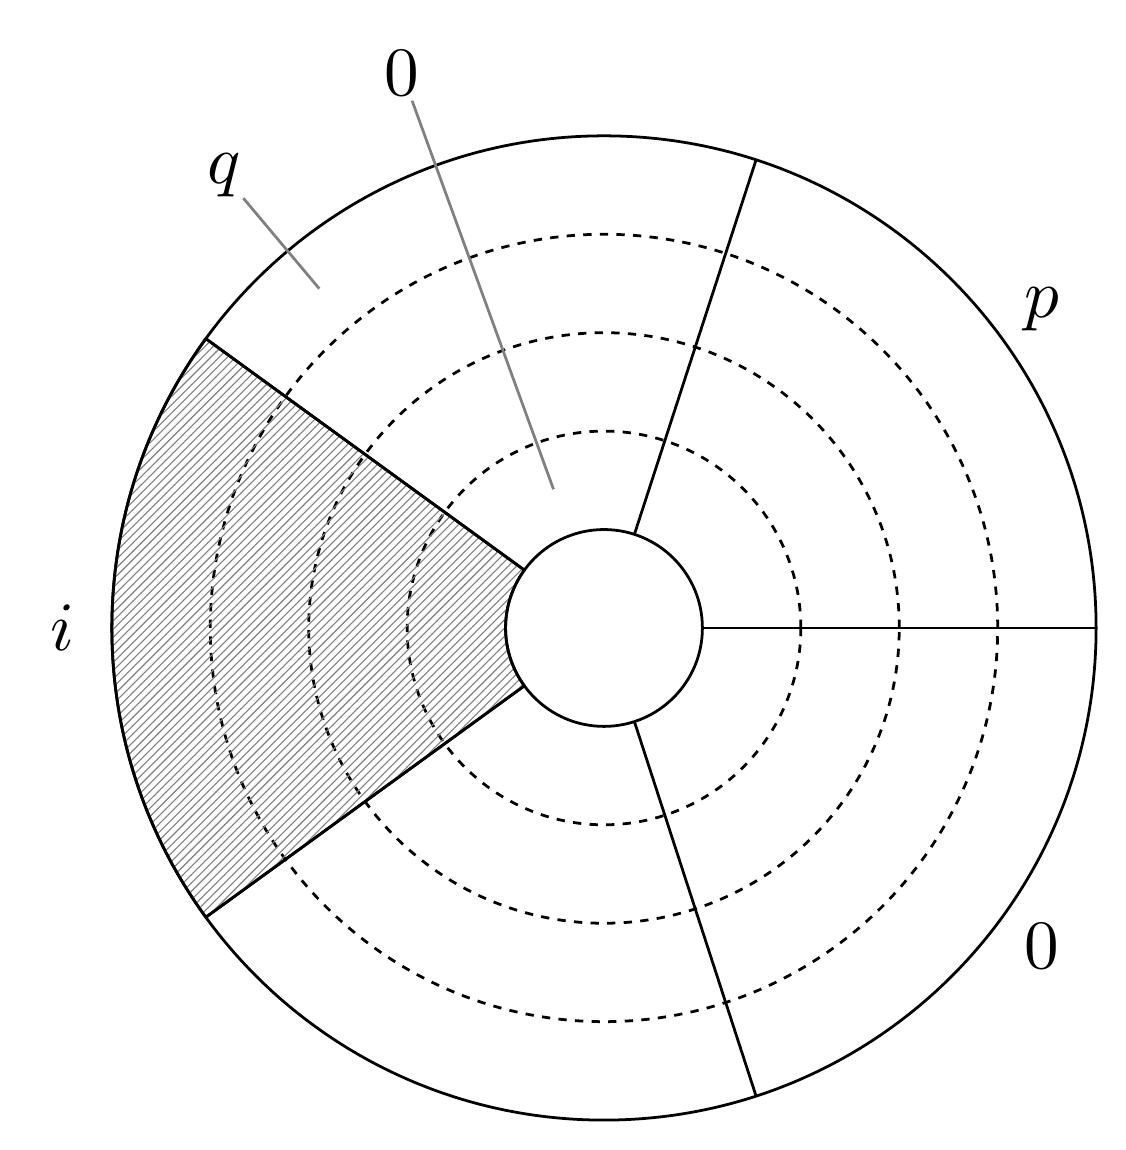
\begin{tikzpicture}[x=1.25cm, y=1.25cm, line width=1pt]

% draw inner and outer circles
\draw[color=black] (0, 0) circle (1);
\draw[color=black] (0, 0) circle (5);

% draw dashed circles
\foreach \i in {2,...,4}
{
    \draw[color=black, dashed] (0, 0) circle (\i);
}

% draw radial lines
\foreach \i in {0,...,4}
{
		\draw (\i * 72 : 1) -- (\i * 72 : 5);
}

% draw nodes
\draw node[scale = 2.5] at (72 * 4 + 36 : 5.5) {$\ul 0$};
\draw node[scale = 2.5] at (72 * 2 + 36 : 5.5) {$\ul i$};
\draw node[scale = 2.5] at (36 : 5.5) {$\ul p$};

\draw node[scale = 2.5] at (110 : 6) {$0$};
\draw[color=black!50] (110 : 5.7) -- (110 : 1.5);
\draw node[scale = 2.5] at (130 : 6) {$q$};
\draw[color=black!50] (130 : 5.7) -- (130 : 4.5);

% draw shaded radial segment
\filldraw[pattern=north east lines, pattern color=gray] (72 * 2 : 1) arc [radius = 1, start angle = 72 * 2, delta angle = 72]
                                                     -- (72 * 3 : 5) arc [radius = 5, start angle = 72 * 3, delta angle = - 72]
                                                     -- cycle;                                                    
\end{tikzpicture}}
\end{minipage}
\end{document}